\documentclass[a4paper]{article}
\usepackage[utf8]{inputenc}
\usepackage[russian,english]{babel}
\usepackage[T2A]{fontenc}
\usepackage[left=10mm, top=20mm, right=18mm, bottom=15mm, footskip=10mm]{geometry}
\usepackage{indentfirst}
\usepackage{amsmath,amssymb}
\usepackage[italicdiff]{physics}
\usepackage{graphicx}
\graphicspath{{images/}}
\DeclareGraphicsExtensions{.pdf,.png,.jpg}
\usepackage{wrapfig}
\usepackage{float}
\usepackage{subcaption}
\usepackage{enumitem}
\usepackage{pdflscape}
\usepackage{caption}
\usepackage{array}
\captionsetup[figure]{name=Рисунок}
\captionsetup[table]{name=Таблица}

\title{\underline{Отчет о выполненой лабораторной работе 5.4.1}}
\author{Воронин Денис, Б04-407}

\begin{document}

\maketitle

\begin{center}
\textbf{\Large Определение энергии $\alpha$ - частицы по величине их пробега в воздухе}
\end{center}

\textbf{Цель работы:} измерить величину пробега $\alpha$ - частицы 3 -мя способами: счетчиком Гейгера, сцинтилляционного счетчика, ионизационной камеры.


\textbf{В работе используются:} торцевой счетчик Гейгера, сцинтилляционный счетчик, ионизационная камера
\section{Теоретические сведения}

\textbf{Радиоактивность} --- самопроизвольный распад ядер с испусканием одной или нескольких частиц.

\textbf{Рад-ть характеризуется}:
\begin{enumerate}
    \item \(t_{\text{протек}}\)
    \item сортом частиц
    \item их энергией
    \item угловой корреляцией
\end{enumerate}

\textbf{Радиоактивные процессы}: \(\alpha, \beta, \gamma\) --- излучения, деление ядер, испускание запаздывающих нейтронов и протонов.

\textbf{\underline{\(\alpha\) --- распад}}

Спонтанному \(\alpha\) --- распаду подвержены только ядра с \(Z > 83\) и \(A = 140 - 160\) (редкоземельные эл-ты)

Периоды полураспада подчиняются \textbf{з-ну Гейгера-Неттола}

Схема: \({}^A_Z X \rightarrow {}^{A-4}_{Z-2} Y + {}^4_2 He\)

\(\alpha\) --- распад эн-ки возможен если:
\[
\Delta E = E_{Z-2}^{A-4} + E_\alpha - E_Z^A > 0
\]
\[
E_{\text{св}}(\alpha) = 28 \text{ МэВ}
\]

Вид пот эн. \(\alpha\) --- распада в ядре и в его окрестности:

\begin{figure}[!hb]
	\centering
	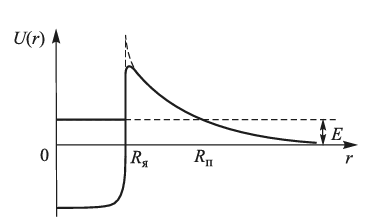
\includegraphics[width=0.3\linewidth]{p1.png}
	\caption{Вид потенциальной энергии альфа - частицы в ядре и в его окрестности}
	\label{pic_2}
\end{figure}

\[
E_n = \frac{2(Z-2)e^2}{r} \text{ --- пот. эн. эл. сил Кулоновского отталкивания}
\]

Проницаемость пот. барьера для \(\alpha\)-частицы с эн-ей \(E\):
\begin{equation}
\ln D = -\frac{2}{\hbar} \int_{R_\alpha}^{R_n} \sqrt{2m_\alpha (U-E)} dr
\tag{1}
\end{equation}

\(R_n\) --- точка поворота (так как в классической физике частица отражалась бы от барьера)

\newpage
Предположим, что $E<<U$ всюду, тогда из (1): 
\[
\begin{aligned}
\ln D &\simeq \frac{2\sqrt{2m}\alpha}{\hbar} \int_{R_a}^{R_n} \sqrt{\frac{2(Z-2)e^2}{r}} \, dr 
= -\mathrm{const} \cdot \int_{R_a}^{R_n} \frac{dr}{\sqrt{r}} \simeq \\
&\simeq -(A\sqrt{R_n} - B) = -A \left( \frac{B}{\sqrt{E}} + C \right),
\end{aligned}
\]

З-он Гейгера --- Неттола:
\begin{equation}
\lg T_{1/2} = \frac{a}{\sqrt{E}} + b
\tag{3}
\end{equation}

Связь \(T_{1/2}\) с эн-ей альфа-частицы, где \(a = 16Z\); \(b = -16 Z^{3/2} - 21.4\)

\(T_{1/2}\) зав-т от эн-ей вылета альфа-частиц:
\begin{itemize}
    \item слабо зав-т от \(Z\)
    \item не зав-т от массового числа ядра
\end{itemize}

\textbf{Константа распада}:
\begin{equation}
\lambda = \frac{\ln 2}{T_{1/2}} = \nu D
\tag{4}
\end{equation}
где \(\nu\) --- число попыток в единицу времени преодолеть барьер

Грубая оценка:
\begin{equation}
\nu = \frac{v}{2R_\text{я}}
\tag{5}
\end{equation}
где \(\vartheta \) --- скорость альфа частицы внутри ядра: \(\vartheta  = \frac{\bar{h}}{m_\alpha R_\text{я}}\)

\(\alpha\) --- распад может происходить с изменением углового момента ядра
\begin{figure}[!hb]
	\centering
	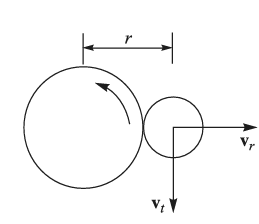
\includegraphics[width=0.3\linewidth]{p2.png}
	\caption{Схема изображения вылета из ядра}
	\label{pic_2}
\end{figure}

ЗСЭ:
\begin{equation}
E = \frac{m_\alpha v^2}{2} + \frac{L^2}{2m_\alpha r^2} + U(r)
\tag{6}
\end{equation}

U(r) - центробежная потенциальная энергия


Увеличение периода полураспада харак-ся величиной:
\begin{equation}
\eta = \frac{\text{ц/б барьер}}{\text{кулон-й барьер}} = \frac{l(l+1)\hbar^2}{2m_\alpha Z(Z-2)e^2r}
\tag{7}
\end{equation}

З-он квантования квадрата момента:
\[
L^2 = l(l+1)\hbar^2
\]

Оценка:
\[
Z=90, \quad R_\text{я} = 10^{-12} \text{ см} \Rightarrow \eta \simeq 0.002 l(l+1)
\]

В лабораторной работе пробег \(\alpha\)-частицв опред-ся 3-мя моделями:
\begin{itemize}
    \item торцевой счётчик Гейгера
    \item сцинтилляционной счетчик
    \item ионизационная камера
\end{itemize}

\[
T_{1/2} \in [10^{-7}; 10^{18} \text{ лет}]
\]
\[
E_\alpha \in (4; 9) \text{ МэВ}
\]

Существует ионизационная потеря в вещ-ве

Приобретенная эн-ки эл-нов при столкновении:
\[
E_e = \frac{p^2}{2m} = \frac{2e^4z^2}{mv^2y^2}
\]

Потеря эн-ии зар-ой частицей:
\begin{equation}
dE(y) = \frac{4\pi n Zz^2 e^4}{mv^2} \frac{dz}{y}
\tag{8}
\end{equation}

Тормозное способ-ть вещ-ва:
\[
\left( \frac{dE}{dx} \right)_{\text{ион}} \simeq \frac{2\pi e^4 z^2}{m v^2} n Z \ln \frac{2 m v^2}{I}
\]

Кривая Брэгга --- зависимость \(dE/dx\) от пути

Длина пробега частицы:
\[
R \propto E^2 = 0.32 E^{3/2}
\]

\(\alpha\)-частица испускается \(^{239}Pu\) с эн. \(\approx 5.15\) МэВ

\section{Экспериментальные установки}

\begin{figure}[htbp]
    \centering
    \begin{minipage}[t]{0.48\linewidth}
        \centering
        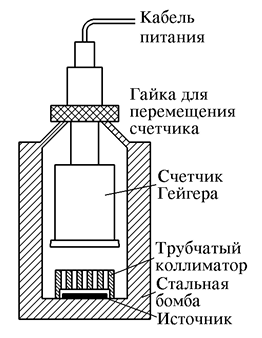
\includegraphics[width=0.5\linewidth]{p3.png}
        \caption{Счетчие Гейгера}
        \label{fig:img1}
    \end{minipage}\hfill
    \begin{minipage}[t]{0.48\linewidth}
        \centering
        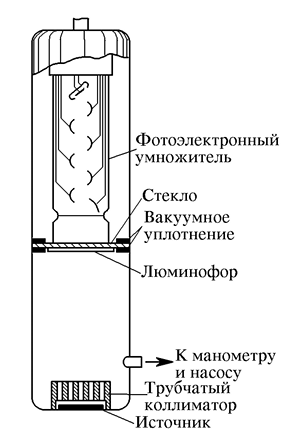
\includegraphics[width=0.5\linewidth]{p4.png}
        \caption{Сцинтилляционный счетчи}
        \label{fig:img2}
    \end{minipage}
    % \caption{Два рисунка рядом}
    \label{fig:both}
\end{figure}

\begin{figure}[!hb]
	\centering
	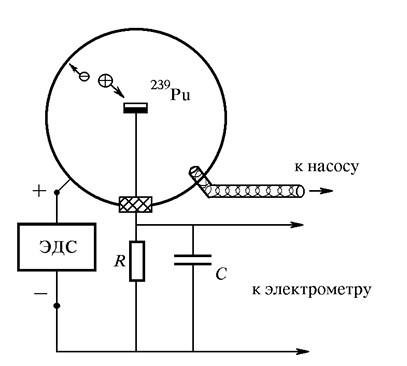
\includegraphics[width=0.3\linewidth]{p5.png}
	\caption{Ионизационная камера}
	\label{pic_2}
\end{figure}

\newpage

\section{Ход работы}

\subsection{Счетчик Гейгера}

Результаты эксперимента представлены в таблице:

\begin{table}[h]
\centering
\caption{Зависимость количества импульсов от координаты с погрешностями}
\begin{tabular}{|c|c|c|c|}
\hline
\textbf{Кол-во импульсов, $N$} & \textbf{$x$, мм} & \textbf{$\sigma x$, мм} & \textbf{$\sigma N = \sqrt{N}$} \\
\hline
905  & 10     & 0{,}5 & 30{,}1 \\
1031 & 11     & 0{,}5 & 32{,}1 \\
1000 & 12     & 0{,}5 & 31{,}6 \\
998  & 13     & 0{,}5 & 31{,}6 \\
919  & 14     & 0{,}5 & 30{,}3 \\
874  & 15     & 0{,}5 & 29{,}6 \\
827  & 15{,}5   & 0{,}5 & 28{,}8 \\
844  & 15{,}75  & 0{,}5 & 29{,}1 \\
713  & 16     & 0{,}5 & 26{,}7 \\
697  & 16{,}25  & 0{,}5 & 26{,}4 \\
550  & 16{,}5   & 0{,}5 & 23{,}5 \\
451  & 16{,}75  & 0{,}5 & 21{,}2 \\
256  & 17     & 0{,}5 & 16{,}0 \\
195  & 17{,}25  & 0{,}5 & 14{,}0 \\
108  & 17{,}5   & 0{,}5 & 10{,}4 \\
62   & 17{,}75  & 0{,}5 & 7{,}9  \\
38   & 18     & 0{,}5 & 6{,}2  \\
43   & 18{,}75  & 0{,}5 & 6{,}6  \\
34   & 19{,}5   & 0{,}5 & 5{,}8  \\
24   & 20{,}25  & 0{,}5 & 4{,}9  \\
\hline
\end{tabular}
\end{table}

Апроксимация проводилась по фомуле: 

\[
f(x) = \frac{A}{1 + e^{\frac{X - X_0}{B}}}.
\]

\begin{figure}[!hb]
	\centering
	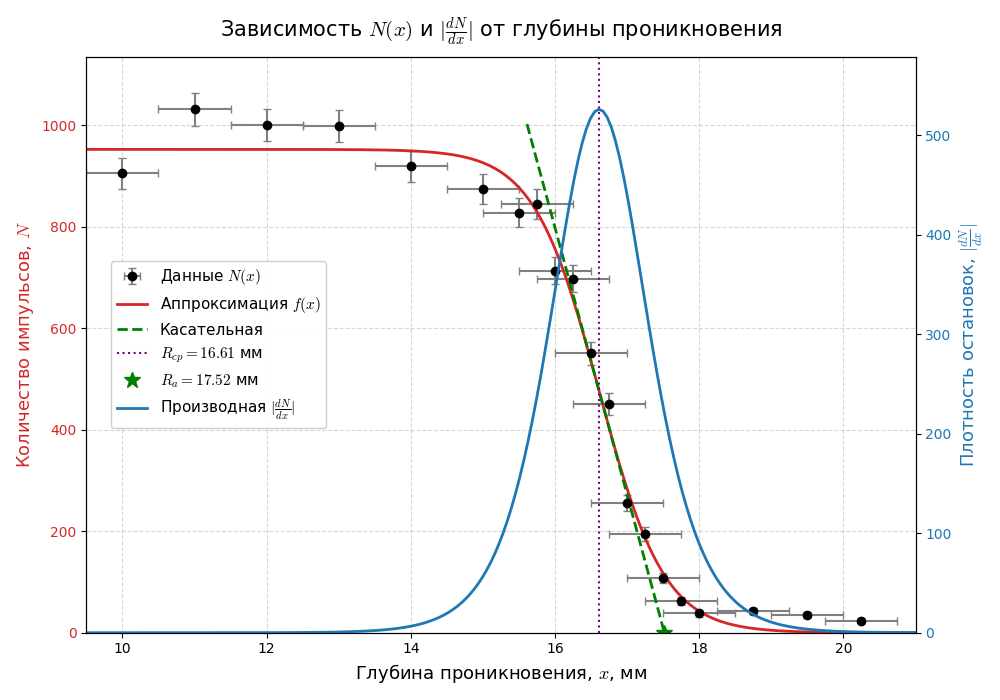
\includegraphics[width=0.8\linewidth]{F1.png}
	\caption{График для счетчика Гейгера}
	\label{pic_2}
\end{figure}

\newpage

\begin{table}[h]
\centering
\caption{Параметры аппроксимации и рассчитанные характеристики}
\begin{tabular}{|l|c|c|c|}
\hline
\textbf{Параметр} & \textbf{Обозначение} & \textbf{Значение} & \textbf{Ед. изм.} \\ \hline
Амплитуда (макс. счет) & \(A\) & \(958 \pm 15\) & имп. \\ \hline
Точка перегиба & \(x_0\) & \(16,61 \pm 0,04\) & мм \\ \hline
Крутизна спада & \(B\) & \(0,455 \pm 0,025\) & мм \\ \hline
Средний пробег & \(R_{cp}\) & \(16,61 \pm 0,04\) & мм \\ \hline
Экстраполированный пробег & \(R_a\) & \(17,52 \pm 0,06\) & мм \\ \hline
Средняя энергия \(\alpha\)-частиц & \(E_{cp}\) & \(2,99 \pm 0,01\) & МэВ \\ \hline
Экстраполированная энергия & \(E_a\) & \(3,11 \pm 0,01\) & МэВ \\ \hline
\end{tabular}
\end{table}

Средний $R_{\mathrm{ср}}$ и экстраполированный $R_{\mathrm{экстр}}$ пробеги определяются следующими уравнениями:
\[
\begin{cases}
N''(R_{\mathrm{ср}}) = 0, \\[8pt]
R_{\mathrm{экстр}} = R_{\mathrm{ср}} + \left| N(R_{\mathrm{ср}}) / N'(R_{\mathrm{ср}}) \right|.
\end{cases}
\]
Энергию можно найти из формулы: $E = (R/0{,}32)^{2/3}$.

Альфа-частицы с энергией около 5~МэВ теряют примерно 100--150~кэВ на каждый микрометр слюды (или $\sim$150~кэВ на 1~мг/см${}^2$).

$5{,}15 - 3{,}11 = 2{,}04$~МэВ энергии.


Тогда толщина пластинки:
\[
t \approx \frac{2{,}04~\text{МэВ}}{0{,}15~\text{МэВ}/\text{мкм}} \approx 13{,}6~\text{мкм}.
\]

\subsection{Сцинтилляционный счетчик}


\begin{table}[h]
\centering
\caption{Данные сцинтилляционного счетчика}
\begin{tabular}{|c|c|c|c|}
\hline
\textbf{$P$, тор} & \textbf{$N$, шт} & \textbf{$\sigma_P$, тор} & \textbf{$\sigma_N = \sqrt{N}$} \\
\hline
745  & 3608 & 7{,}5 & 60{,}1 \\
700  & 2931 & 7{,}5 & 54{,}1 \\
675  & 2632 & 7{,}5 & 51{,}3 \\
650  & 2170 & 7{,}5 & 46{,}6 \\
625  & 1677 & 7{,}5 & 41{,}0 \\
600  & 1392 & 7{,}5 & 37{,}3 \\
575  & 850  & 7{,}5 & 29{,}2 \\
552  & 537  & 7{,}5 & 23{,}2 \\
527  & 242  & 7{,}5 & 15{,}6 \\
500  & 37   & 7{,}5 & 6{,}1  \\
475  & 5    & 7{,}5 & 2{,}2  \\
\hline
\end{tabular}
\end{table}


\begin{table}[h]
\centering
\caption{Параметры аппроксимации и вычисленные значения энергии}
\begin{tabular}{|l|c|c|c|}
\hline
\textbf{Параметр} & \textbf{Обозначение} & \textbf{Значение} & \textbf{Ед. изм.} \\
\hline
Нижняя асимптота              & $B_1$   & $\approx 0 \pm 5$       & имп.   \\
Верхняя асимптота             & $B_2$   & $3810 \pm 45$           & имп.   \\
Точка перегиба (среднее)      & $P_0$   & $135{,}4 \pm 1{,}5$     & торр   \\
Параметр крутизны             & $dP$    & $40{,}5 \pm 1{,}2$      & торр   \\
Среднее давление              & $P_{\text{ср}}$ & $135{,}4 \pm 1{,}5$ & торр \\
Экстраполированное давление   & $P_a$   & $216{,}3 \pm 2{,}5$     & торр   \\
\hline
\end{tabular}
\end{table}

\textbf{Пробег и Энергия $R_{\text{cp}}$ и $E_{\text{cp}}$:} количесвто веществ в препарате 12,2 мкг 
\[
R_{\mathrm{ср}}  \approx 1{,}56 \pm 0,02 ~\text{см}.
\]

\[
E_{\mathrm{ср}}  \approx 2{,}87 \pm 0,02 ~\text{МэВ}.
\]

\textbf{ $R_a$ и $E_a$:}
\[
R_a \approx 2{,}50 \pm 0,02~\text{см}.
\]

\[
E_a \approx 3{,}93 \pm 0,02~\text{МэВ}.
\]

\newpage

\begin{figure}[!hb]
	\centering
	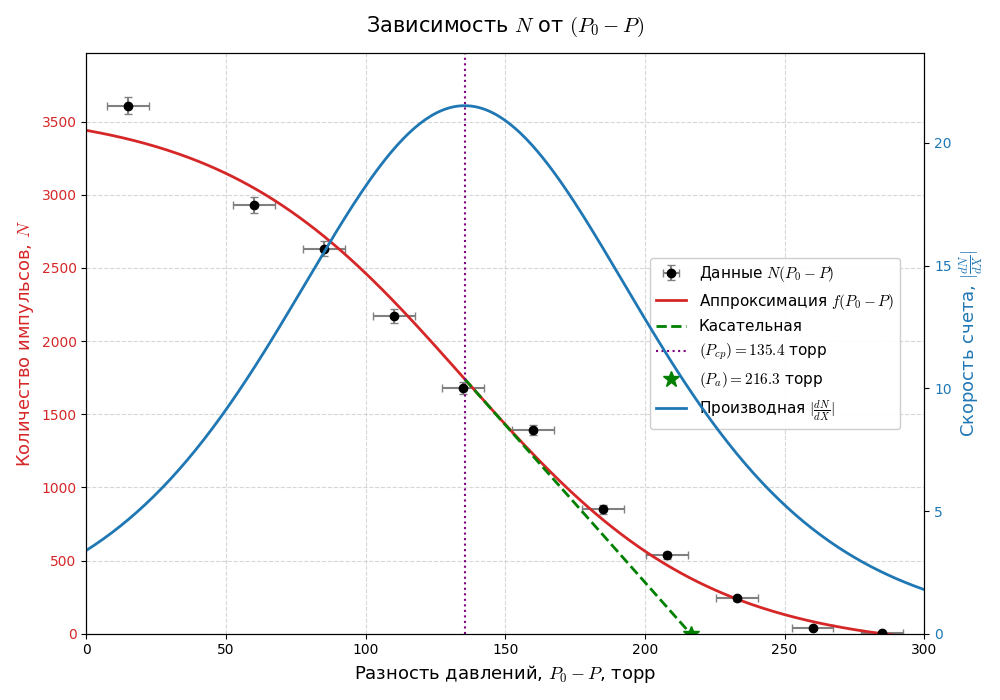
\includegraphics[width=0.7\linewidth]{F2.png}
	\caption{График для сцинтиляционного счетчика}
	\label{pic_2}
\end{figure}

\subsection{Ионизационная камера}

\begin{figure}[!hb]
	\centering
	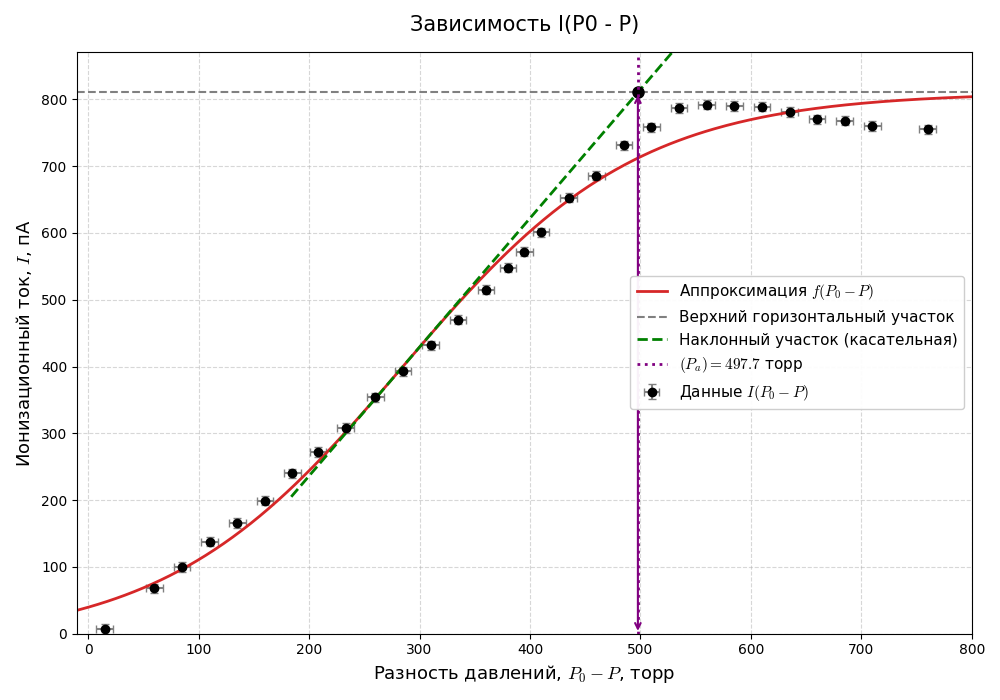
\includegraphics[width=0.8\linewidth]{F3.png}
	\caption{Ионизационная камера}
	\label{pic_2}
\end{figure}

\[
R_a \approx 3{,}19 \pm 0,09~\text{см}.
\]

\[
E_a \approx 4{,}63 \pm 0,12~\text{МэВ}.
\]

\newpage

\begin{table}[h]
\centering
\caption{Зависимость тока ионизации от давления}
\begin{tabular}{|c|c|c|c|}
\hline
\textbf{$P$, торр} & \textbf{$I_{\text{ион}}$, пА} & \textbf{$\sigma_P$, тор} & \textbf{$\sigma_I$, пА} \\
\hline
745  & 7   & 7{,}5 & 7 \\
700  & 68  & 7{,}5 & 7 \\
675  & 100 & 7{,}5 & 7 \\
650  & 138 & 7{,}5 & 7 \\
625  & 166 & 7{,}5 & 7 \\
600  & 199 & 7{,}5 & 7 \\
575  & 240 & 7{,}5 & 7 \\
552  & 272 & 7{,}5 & 7 \\
527  & 308 & 7{,}5 & 7 \\
500  & 354 & 7{,}5 & 7 \\
475  & 393 & 7{,}5 & 7 \\
450  & 432 & 7{,}5 & 7 \\
425  & 470 & 7{,}5 & 7 \\
400  & 515 & 7{,}5 & 7 \\
380  & 548 & 7{,}5 & 7 \\
365  & 572 & 7{,}5 & 7 \\
350  & 601 & 7{,}5 & 7 \\
325  & 653 & 7{,}5 & 7 \\
300  & 686 & 7{,}5 & 7 \\
275  & 731 & 7{,}5 & 7 \\
250  & 758 & 7{,}5 & 7 \\
225  & 787 & 7{,}5 & 7 \\
200  & 792 & 7{,}5 & 7 \\
175  & 790 & 7{,}5 & 7 \\
150  & 789 & 7{,}5 & 7 \\
125  & 781 & 7{,}5 & 7 \\
100  & 770 & 7{,}5 & 7 \\
75   & 768 & 7{,}5 & 7 \\
50   & 760 & 7{,}5 & 7 \\
0    & 755 & 7{,}5 & 7 \\
\hline
\end{tabular}
\end{table}


\section{Выводы}

1. При проведении измерения энергии альфа частиц по величине их пробега с помощью счетчика Гейгера получили значение энегрии на 2 МэВ ниже (3,11 МэВ), чем ожидалось (5,15 МэВ).
Это связано с тем, что альфа частица тратит часть своей энергии на преоление пленки источника и слюдяной пластинки на счетчике. В счетчике Гейгера самые большие потери.


2. При измерении с помощью сцинтилляционного счетчкика получили энергию чуть повыше (3,93 МэВ). Это связано с тем что на сцинтилятор покрыт защитным светоотражающим слоем. Поэтому потери есть, но не такие большие, как в счетчике Гейгера.


3. В 3 способе получили энергию близкую к табличной (4,63 МэВ). Это связано с минимальной толщиной входного окна и высокой чувствительностью к ионизации.

\end{document}